\documentclass[notes,blackandwhite,mathsans]{beamer}

\usepackage{amsmath}
\usepackage{amssymb}
\usepackage{graphicx}
\usepackage{fancybox}
\usepackage{booktabs}
\usepackage{multirow,pxfonts}
\usepackage{cmbright}
\usepackage{color}
\usepackage{xcolor}
\usepackage{changepage}

\usepackage[T1]{fontenc}
\fontencoding{T1}  
\usepackage[utf8]{inputenc}


\usefonttheme{default}
\setbeamercovered{invisible}
\beamertemplatenavigationsymbolsempty

\makeatletter
\setbeamertemplate{footline}
{
  \leavevmode
  \hbox{
  \begin{beamercolorbox}[wd=0.97\paperwidth,ht=2.25ex,dp=2ex,right]{}
{\color{mcxs3} \insertframenumber{} / \inserttotalframenumber}
  \end{beamercolorbox}}%
}


\definecolor{mcxs1}{HTML}{05386B}
\definecolor{mcxs2}{HTML}{379683}
\definecolor{mcxs3}{HTML}{5CDB95}
\definecolor{mcxs4}{HTML}{8EE4AF}
\definecolor{mcxs5}{HTML}{EDF5E1}
\setbeamercolor{frametitle}{fg=mcxs2}
\AtBeginDocument{\color{mcxs1}}

%\setbeamercolor{itemize text}{fg=mcxs5}
\setbeamercolor{itemize item}{fg=mcxs1}
\setbeamercolor{itemize subitem}{fg=mcxs2}
\setbeamercolor{enumerate item}{fg=mcxs1}
\setbeamercolor{description item}{fg=mcxs1}

%\setbeamertemplate{itemize item}[triangle]
%\setbeamertemplate{itemize subitem}[circle]






\begin{document}
%\fontfamily{pag}\selectfont
%\setbeamerfont{title}{family=\fontfamily{pag}\selectfont}
%\setbeamerfont{frametitle}{family=\fontfamily{pag}\selectfont}
%\setbeamerfont{framesubtitle}{family=\fontfamily{pag}\selectfont}






{\setbeamercolor{background canvas}{bg=mcxs2}
\begin{frame}

\vspace{1cm}
\begin{tabular}{rl}
&\textbf{\LARGE\color{mcxs1} Macroeconometrics}\\[6ex]
\textbf{\color{mcxs3}\Large Lecture 6}&\textbf{\Large\color{mcxs3}Macroeconometrics research themes}\\[19ex]
&\textbf{\color{mcxs1} Tomasz Wo\'zniak}\\[1ex]
&{\small\color{mcxs3} Department of Economics}\\
&{\small\color{mcxs3}University of Melbourne}
\end{tabular}

\end{frame}
}






{\setbeamercolor{background canvas}{bg=mcxs2}
\begin{frame}

%\bigskip\textbf{\color{mcxs3}What's macroeconometrics?}

\bigskip\textbf{\color{mcxs3}Forecasting with Bayesian VARs}

\bigskip\textbf{\color{mcxs1}Assessing policy effects with Structural VARs}

\bigskip\textbf{\color{mcxs3}Trend and cycle analysis with Unobserved Component models}

\end{frame}
}














{\setbeamercolor{background canvas}{bg=mcxs3}
\begin{frame}

\begin{adjustwidth}{-0.5cm}{0cm}
%\FlushLeft
\vspace{8.3cm}\Large
\textbf{{\color{mcxs2}Forecasting with} {\color{mcxs1}Bayesian VARs}}
\end{adjustwidth}

\end{frame}
}




\begin{frame}{Forecasting with Bayesian VARs}

\textbf{Baseline model: Vector Autoregression}
\begin{align*}
y_t &= A_1 y_{t-1} + \dots + A_p y_{t-p}  + \mu_0 + \epsilon_t\\[1ex]
\epsilon_t|Y_{t-1} &\sim iid\left(\mathbf{0}_N,\Sigma\right)\\
\end{align*}

\begin{description}
\item[System modelling] {\color{mcxs2}-- all variables are endogenous} 
\item[Dynamics] {\color{mcxs2}-- captures system dynamics of the variables} 
\item[Forecasting] {\color{mcxs2}-- a go to model for predictive applications} 
\item[Extensions] {\color{mcxs2} capturing important data features improve forecasting precision}
\end{description}
\end{frame}




\begin{frame}{Forecasting with Bayesian VARs}

\bigskip\textbf{Objective: Density forecasting performance evaluation}
\begin{align*}
p(y_{T+h}\mid Y_{T})
\end{align*}

\centering
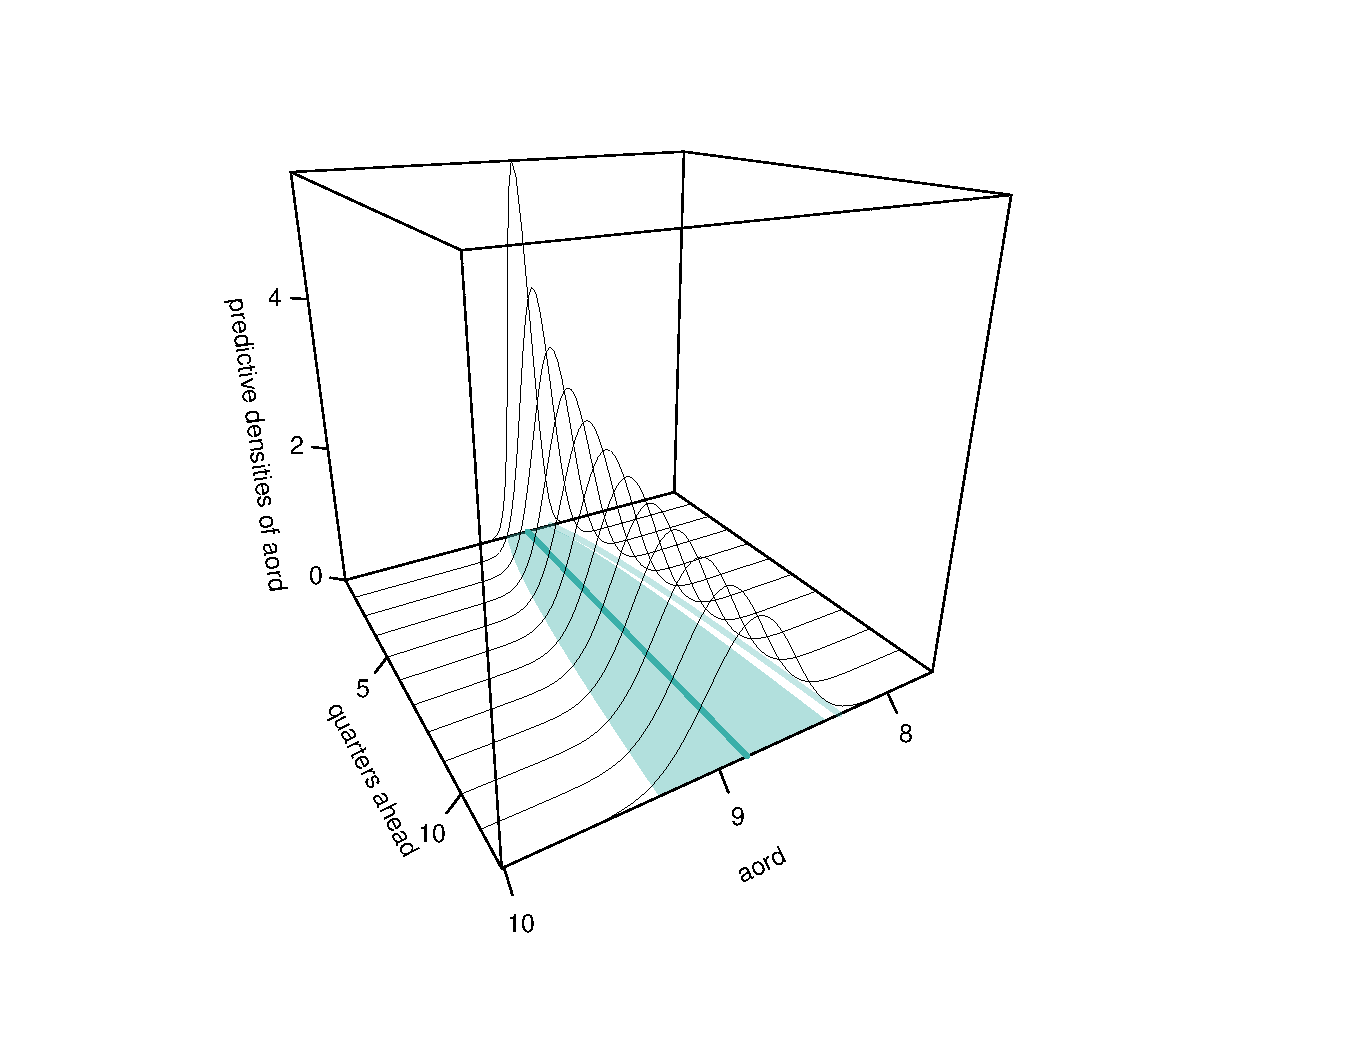
\includegraphics[scale=0.4, trim=0cm 0cm 0cm 1cm]{grphs/06density}

\end{frame}




\begin{frame}{Forecasting with Bayesian VARs}

\centering
\bigskip\textbf{Method: Recursive forecasting exercise}

\bigskip
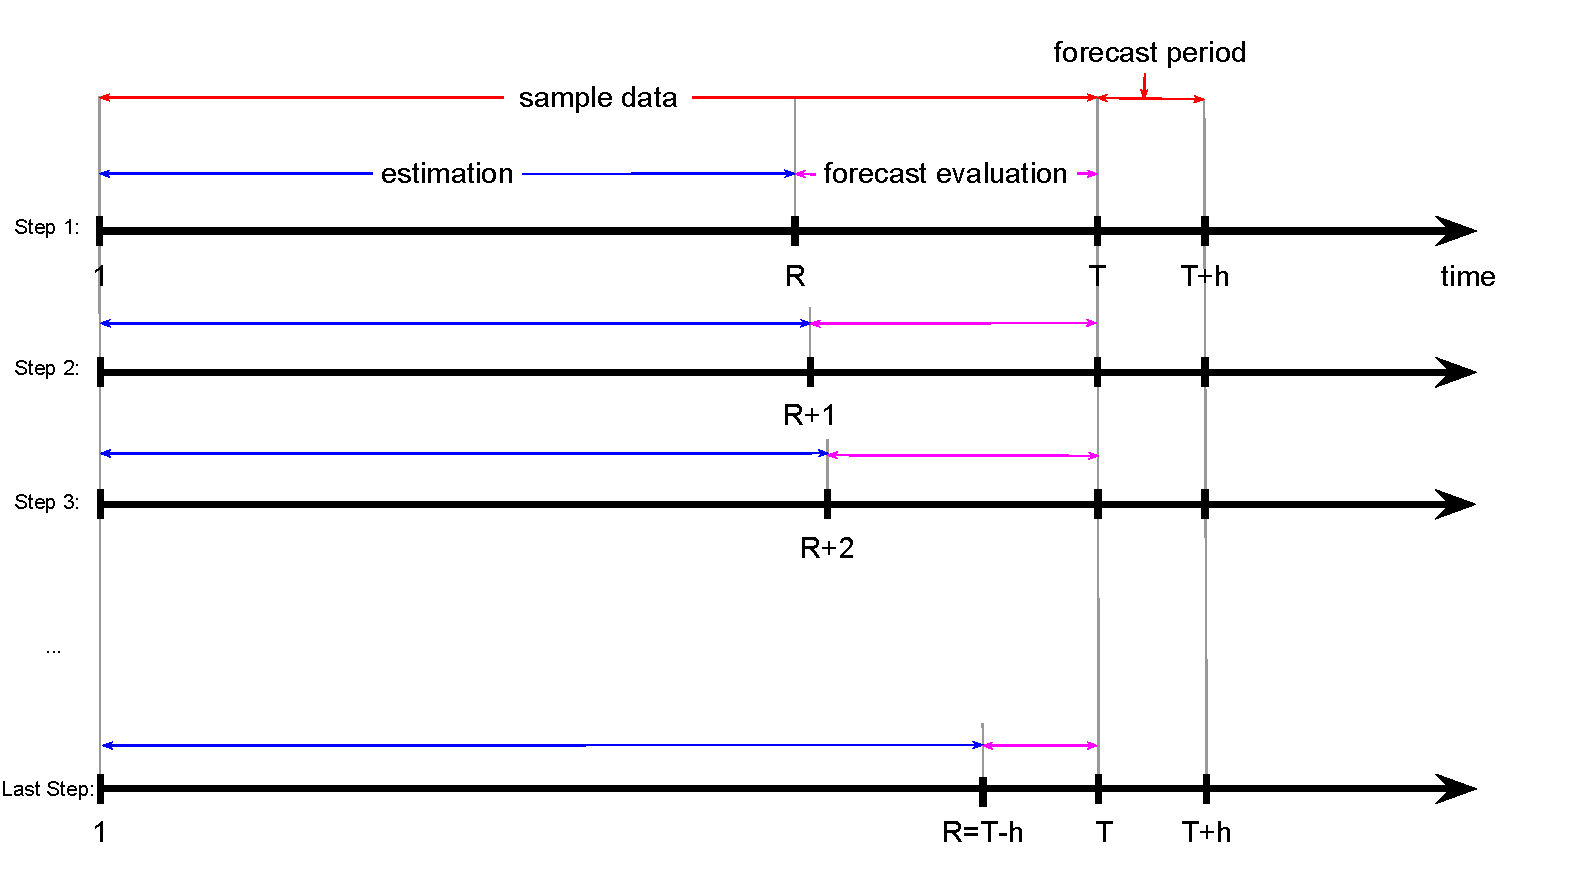
\includegraphics[scale=0.4]{grphs/06recursive}
\end{frame}





\begin{frame}{Forecasting with Bayesian VARs}
\textbf{Data set examples. }
\bigskip
\begin{description}
\item[Fat data] {\color{mcxs2}of 117 quarterly macro variables for Australia} \\ [1ex]
\item[Bond yield curve modelling] {\color{mcxs2}using daily/monthly interest rates} \\ [1ex]
\item[Small-open economy] {\color{mcxs2}forecasting with a foreign sector} \\ [1ex]
\item[] {\color{mcxs2} }
\end{description}
\end{frame}



\begin{frame}{Forecasting with Bayesian VARs}
\textbf{Potential model extensions. }
\bigskip
\begin{description}
\item[Common heteroskedasticity] {\color{mcxs2}for all variables}\\ [1ex]
\item[Non-normal error term] {\color{mcxs2}via gamma-scale mixtures}\\ [1ex]
\item[Estimated prior shrinkage] {\color{mcxs2}of the Minnesota prior}\\ [1ex]
\item[] {\color{mcxs2} }
\end{description}
\end{frame}










{\setbeamercolor{background canvas}{bg=mcxs2}
\begin{frame}

\begin{adjustwidth}{-0.5cm}{0cm}
%\FlushLeft
\vspace{8.3cm}\Large
\textbf{{\color{mcxs3}Assessing policy effects with  } {\color{mcxs1}Structural VARs}}
\end{adjustwidth}

\end{frame}
}





\begin{frame}{Assessing policy effects with Structural VARs}

\textbf{Structural Vector Autoregressions.}
\begin{align*}
y_t &= A_1 y_{t-1} + \dots + A_p y_{t-p}  + \mu_0 + \epsilon_t\\[1ex]
B\epsilon_t &= u_t \\[1ex]
u_t|Y_{t-1} &\sim iid\left(\mathbf{0}_N,I_N\right)\\
\end{align*}

\begin{description}
\item[Structural] {\color{mcxs2}relationships are explicitly modelled} 
\item[Economic theory] {\color{mcxs2}informs identification of structural shocks} 
\item[Dynamic causal effects] {\color{mcxs2}can be estimated and interpreted} 
\item[Policy decision-making] {\color{mcxs2}is based on evidence provided by SVARs}
\end{description}
\end{frame}





\begin{frame}{Assessing policy effects with Structural VARs}

\textbf{Objective: identification of a structural shock and its effects}
\bigskip
\begin{description}
\item[Identification via restrictions] {\color{mcxs2}leading to fast estimation} \\[1ex]
\item[Identification via sign restrictions] {\color{mcxs2}that are less controversial} \\[1ex]
\item[Identification via heteroskedasticity] {\color{mcxs2}using data properties} 
\end{description}
\end{frame}





\begin{frame}{Assessing policy effects with Structural VARs}

\textbf{Method: impulse response analysis}

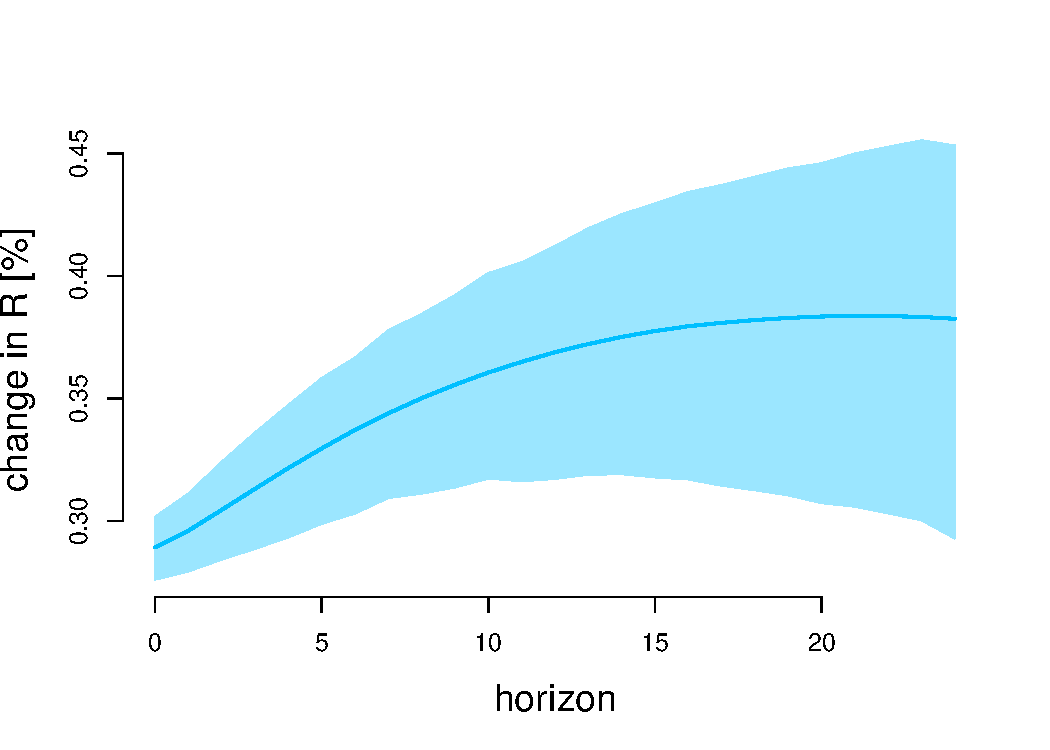
\includegraphics[scale=0.3]{grphs/06irf-33}
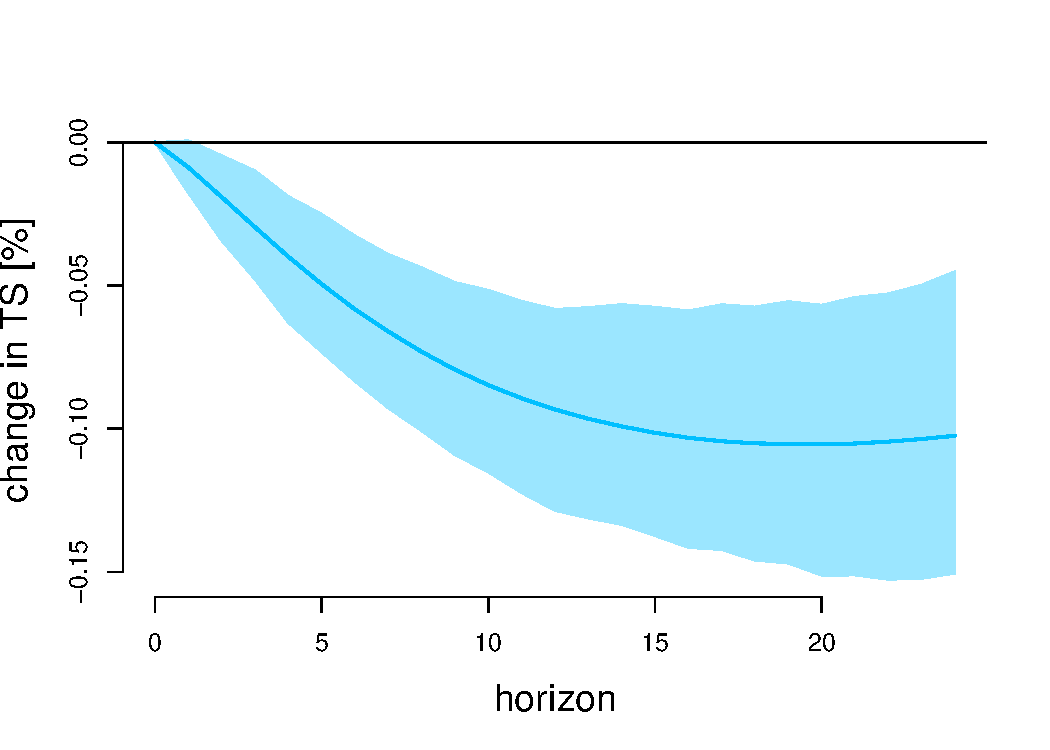
\includegraphics[scale=0.3]{grphs/06irf-43}
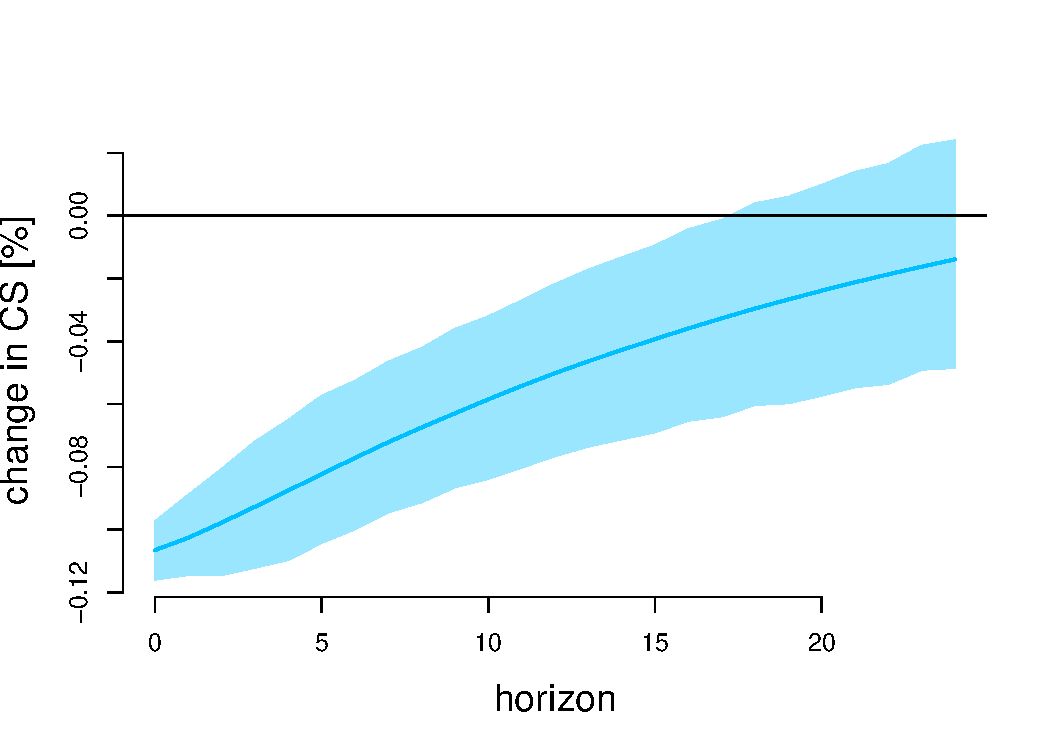
\includegraphics[scale=0.3]{grphs/06irf-63}
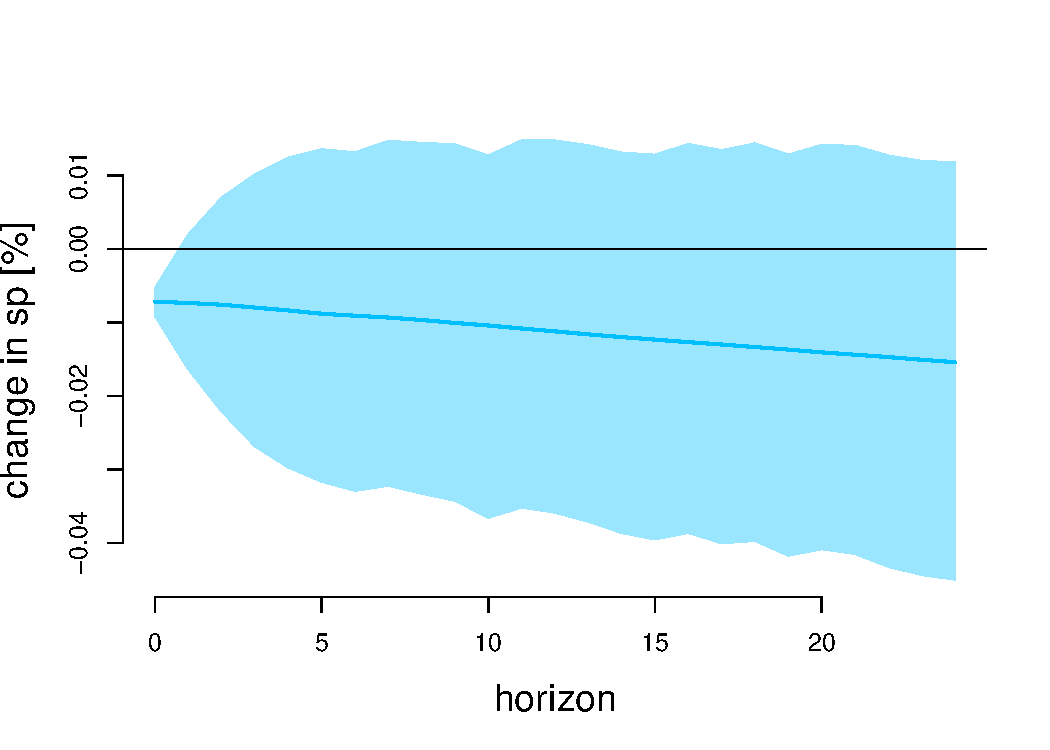
\includegraphics[scale=0.3]{grphs/06irf-73}

\end{frame}



\begin{frame}{Assessing policy effects with Structural VARs}

\textbf{Method: forecast error variance decomposition}

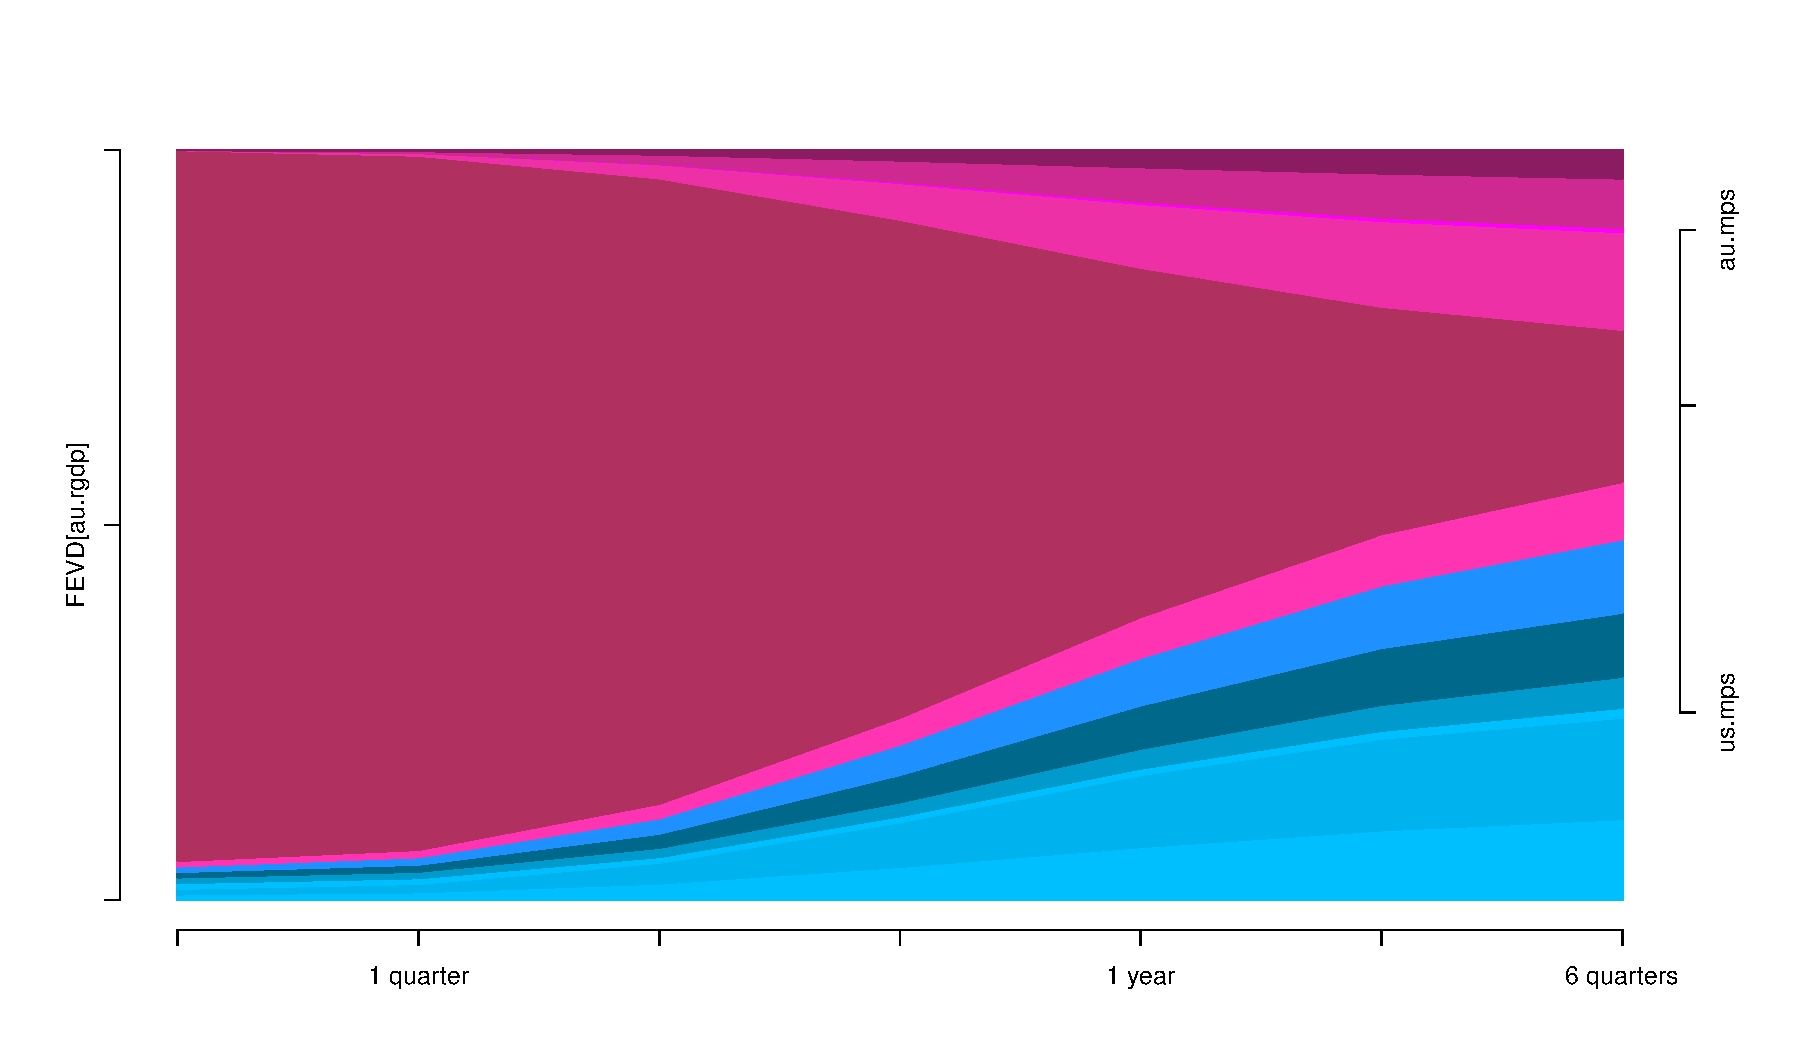
\includegraphics[scale=0.35]{grphs/06fevd}

\end{frame}





{\setbeamercolor{background canvas}{bg=mcxs3}
\begin{frame}

\begin{adjustwidth}{-0.6cm}{0cm}
%\FlushLeft
\vspace{8.3cm}\Large
\textbf{{\color{mcxs2}Trend and cycle analysis with } {\color{mcxs1}UC models}}
\end{adjustwidth}

\end{frame}
}







\begin{frame}{Trend and cycle analysis with UC models}

\bigskip\textbf{Unobserved Component Models.}
\begin{align*}
y_t &= \tau_t + \epsilon_t\\[1ex]
\tau_t &= \mu + \tau_{t-1} + \eta_t \\[1ex]
\epsilon_t &= \alpha_1 \epsilon_{t-1} + \dots +  \alpha_p \epsilon_{t-p} + e_t \\[1ex]
\eta_t|Y_{t-1} &\sim iid\mathcal{N}\left(0,\sigma_\eta^2\right)\\[1ex]
e_t |Y_{t-1} &\sim iid\mathcal{N}\left(0,\sigma_e^2\right)
\end{align*}

\begin{description}
\item[Trend and cycle] {\color{mcxs2}decomposition of a variable} 
\item[Long-run trend] {\color{mcxs2}is highly-persistent} 
\item[Oscillating cycle] {\color{mcxs2}captures short-term dynamics} 
\item[Inflation trend analysis] {\color{mcxs2}and output gap estimation are the main applications}
\end{description}
\end{frame}







\begin{frame}{Trend and cycle analysis with UC models}

\bigskip\textbf{Objective: inflation trend and cycle analysis.}

\centering
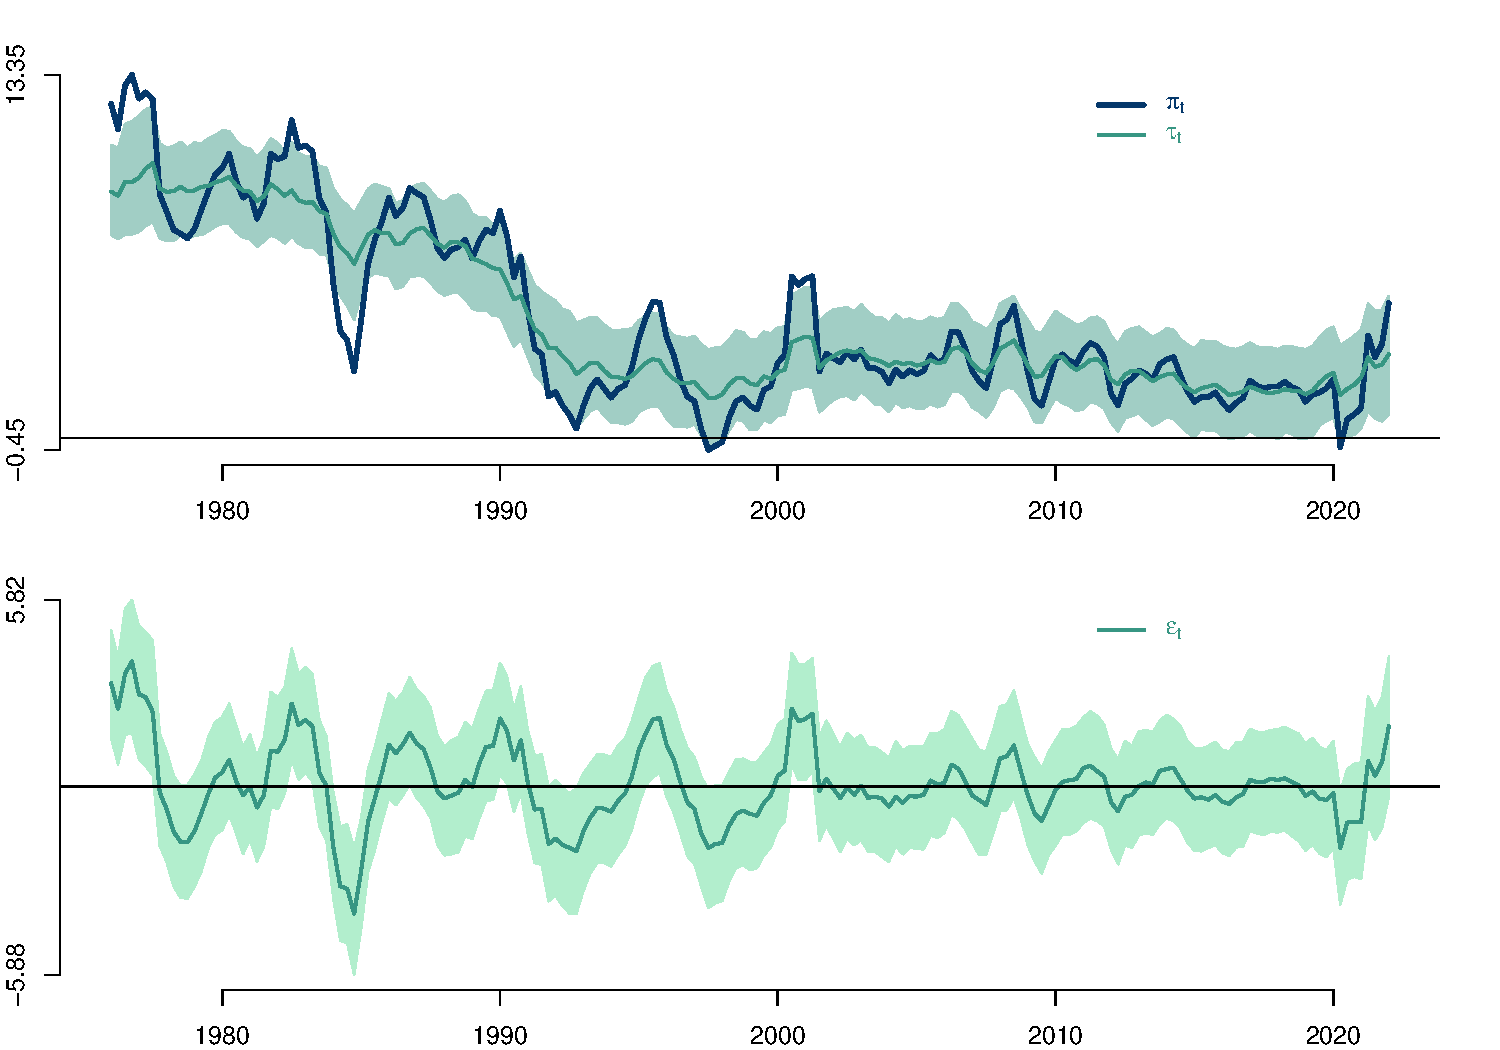
\includegraphics[scale=0.4]{grphs/06trend}
\end{frame}







\begin{frame}{Trend and cycle analysis with UC models}

\bigskip\textbf{Heteroskedastic Model.}
\begin{align*}
y_t &= \tau_t + \epsilon_t\\[1ex]
\tau_t &= \mu + \tau_{t-1} + \eta_t \\[1ex]
\epsilon_t &= \alpha_1 \epsilon_{t-1} + \dots +  \alpha_p \epsilon_{t-p} + e_t \\[1ex]
\eta_t|Y_{t-1} &\sim iid\mathcal{N}\left(0,{\color{mcxs2}\sigma_{\eta.t}^2}\right)\\[1ex]
e_t |Y_{t-1} &\sim iid\mathcal{N}\left(0,{\color{mcxs2}\sigma_{e.t}^2}\right)
\end{align*}
\end{frame}







\begin{frame}{Trend and cycle analysis with UC models}

\bigskip\textbf{Time-varying trend.}
\begin{align*}
y_t &= \tau_t + \epsilon_t\\[1ex]
\tau_t &= {\color{mcxs2}\mu_t} + \tau_{t-1} + \eta_t \\[1ex]
{\color{mcxs2}\mu_t} &{\color{mcxs2}= \mu_{t-1} + m_t} \\[1ex]
\epsilon_t &= \alpha_1 \epsilon_{t-1} + \dots +  \alpha_p \epsilon_{t-p} + e_t \\[1ex]
\eta_t|Y_{t-1} &\sim iid\mathcal{N}\left(0,\sigma_\eta^2\right)\\[1ex]
e_t |Y_{t-1} &\sim iid\mathcal{N}\left(0,\sigma_e^2\right)\\[1ex]
{\color{mcxs2}m_t |Y_{t-1}} &{\color{mcxs2}\sim iid\mathcal{N}\left(0,\sigma_m^2\right)}
\end{align*}

\end{frame}








\begin{frame}{Trend and cycle analysis with UC models}

\bigskip\textbf{Common factor.}
\begin{align*}
{\color{mcxs2}y_{n.t}} &= \tau_t + {\color{mcxs2}\epsilon_{n.t}}\\[1ex]
{\color{mcxs2}n}&{\color{mcxs2}= 1,\dots,N}\\[1ex]
\tau_t &= \mu + \tau_{t-1} + \eta_t \\[1ex]
\epsilon_t &= \alpha_1 \epsilon_{t-1} + \dots +  \alpha_p \epsilon_{t-p} + e_t \\[1ex]
\eta_t|Y_{t-1} &\sim iid\mathcal{N}\left(0,\sigma_\eta^2\right)\\[1ex]
e_t |Y_{t-1} &\sim iid\mathcal{N}\left(0,\sigma_e^2\right)
\end{align*}

\end{frame}












{\setbeamercolor{background canvas}{bg=mcxs4}
\begin{frame}{}

\bigskip
\begin{center}
\LARGE\textbf{The choice is yours!}
\end{center}



\end{frame}
}





\end{document} 